
\chapter{Il comportamento degli utenti}

	Nel 1990 e 1991 si sono effettuati diversi studi sul comportamento degli utenti con metodologie varie. Da questi è sorto che per ogni tipo di \emph{media} l'uomo mette in atto delle regole ben precise. 
	Vedremo un esempio di \emph{media} classico, il perché le sue regole \textbf{non} sono da riutilizzare nel web, quali sono le differenze e quali strumenti abbiamo a disposizione per diminuire gli sforzi dell'utente.
	
	\section{Un media classico: il giornale}
	
		Nel giornale la principale fonte di attrazione è costituita dalle immagini e foto. Più colorate sono, più per lo \emph{scanning} quel blocco è fonte di informazione.
		
		\subsection{L'importanza delle immagini}
		
			Sui giornali le immagini vincono sul testo 80 a 20. I pezzi di testo accompagnati da immagini infatti risultano quelli più letti. \textbf{L'immagine più grande} è il primo \textbf{punto d'entrata} e d'attrazione primaria per invogliare l'utente alla lettura, inoltre in un giornale due pagine aperte sono percepite come un'unica grande pagina.
		
	\section{Il web}
	
		Alla luce di queste informazioni del comportamento tenuto dagli utenti con i giornali si può forse pensare che per le pagine web sia lo stesso. Non è così! La modalità di lettura differisce ma non solo, anche lo spostamento dell'attenzione ha un comportamento diverso come vediamo in figura ~\ref{fig:FasceDAttenzione2}.
		
		\begin{figure} [h]
				\centering
				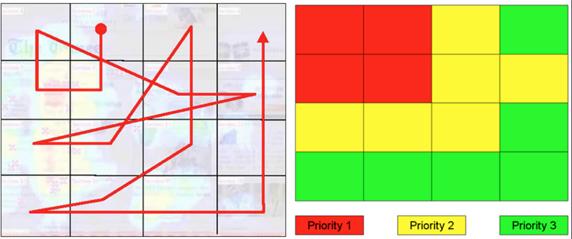
\includegraphics[width=\textwidth]{images/IlComportamentoDegliUtenti-FasceDAttenzione2}
				\caption[Il comportamento degli utenti - Movimento utente e zone calde pagina]{Il comportamento degli utenti - Movimento dell'utente e zone "calde" di una pagina}
				\label{fig:FasceDAttenzione2}
		\end{figure}
		
		\subsection{Fasce d'attenzione}
		
			Per misurare il movimento fatto da utenti in una pagina web si usa la tecnica del \emph{eye tracking} da cui si ricava una termografia di una pagina dove le zone calde corrispondono alle zone a cui l'utente dedica più tempo, mentre quelle fredde corrispondono alle zone che non vede affatto se non nella prima fase di \emph{scanning}. Le diverse termografie classiche indicano che il \textbf{punto d'entrata} di una pagina web è \textbf{in alto a sinistra}. Le fasce d'attenzione risultano quindi avere una forma a \emph{F} o a \emph{cono gelato} come si può notare nella figura ~\ref{fig:FasceDAttenzione}.
			Nella maggioranza dei casi per ogni schermata della stessa pagina abbiamo una forma a \emph{F} nel punto in cui avviene lo \emph{scroll} si ha invece il \emph{blind spot} un punto cieco che non sarà mai visualizzato.
			
			\begin{figure} [h]
				\centering
				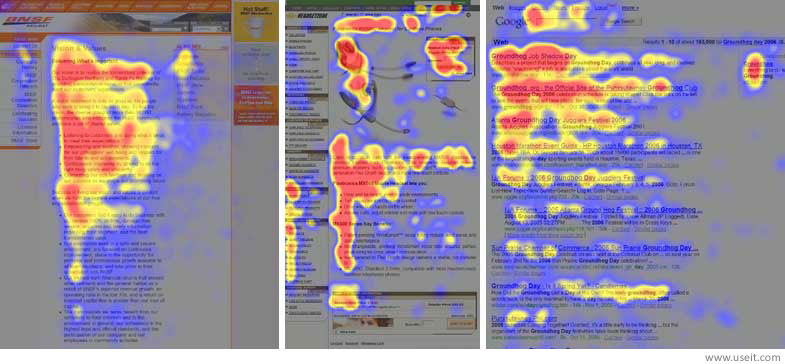
\includegraphics[trim={0 0 0 0}, width=\textwidth]{images/IlComportamentoDegliUtenti-FasceDAttenzione}
				\caption[Il comportamento degli utenti - Termografie]{Il comportamento degli utenti - Esempi di termografie}
				\label{fig:FasceDAttenzione}
			\end{figure}
		
		\subsection{L'importanza del testo}
			Al contrario dei giornali il testo è molto più rilevante rispetto alle immagini nel web. Per sfruttare questo ecco alcuni consigli per migliorare una pagina web.
			\begin{itemize}
				\item Il punto d'attrazione (in alto a sinistra) necessita di testo, il logo deve essere sempre accompagnato da qualche scritta magari che risponda all'asse What.
				\item Il testo su una singola colonna è meglio che su più colonne come nei giornali (l'effetto è molto simile alle liste \emph{itemize} orizzontali).
				\item Le \emph{keyword} messe vicine diluiscono l'importanza data nello \emph{scan}.
				\item Il \emph{bold} non basta per evidenziare le parole chiave. Meglio usare anche la sottolineatura (come un hyperlink) e ingrandire il \emph{font} o meglio ancora separare la o le \emph{keyword} in una riga a parte (una sorta di mini titolo).
			\end{itemize}
		
			\subsubsection{Paragrafi e titoli}
				Un altro utile accorgimento per sfruttare l'importanza del testo è quello di dividere i grandi blocchi di testo in paragrafi corti (rispetto a quelli lunghi attraggono alla lettura quasi il doppio). Lo stesso possiamo dire dei titoli, più sono corti meglio è. Inoltre più un testo è spezzato in piccoli paragrafi più gli utenti sono incoraggiati a leggerlo rilassando i timer (suggerimento valido anche nelle mail).
				Sfruttare il \emph{blurp}, cioè aggiungere ad ogni titolo una mini descrizione per migliorare l'attrazione dell'intera pagina. I \emph{blurp} offrono vantaggi:
				\begin{itemize}
					\item rilassano i timer, ma non cambiano la voglia di proseguire nella navigazione del sito.
					\item aumentano il tasso di ritorno della pagina.
				\end{itemize}
				Il contenuto del \emph{blurp} non è un blocco unico ma può essere suddiviso in parti per cui ha una sua struttura e una sua termografia, per questo motivo le parole fondamentali devono stare alla sinistra del \emph{blurp}.
			
		\subsection{Pagine grasse o magre?}
			Per pagina grassa si intende una pagina web con contenuto più spaziato mentre con la pagina snella una pagina con contenuto più compatto. Dalle analisi è emerso che la pagina grassa funziona peggio. Bisogna infatti porre molta attenzione al separare il testo in paragrafi perché si può incorrere nel \emph{diluited design}. La spaziatura e la separazione portano ad uno \emph{scanning} più veloce ma ciò funziona male nelle pagine ricche di contenuto testuale. In generale:
			\begin{itemize}
				\item la \textbf{pagina grassa} è da preferire in quelle pagine di navigazione con link e poco \emph{scroll};
				\item la \textbf{pagina magra} invece è da preferire in quelle pagine con molto contenuto e tanto \emph{scroll}.
			\end{itemize}
		
		\subsection{Immagini nel web}
			Abbiamo visto che le immagini nel web hanno un ruolo marginale rispetto al testo difatti un'immagine affiancata ad un testo perde quasi tutta l'attenzione. Nonostante questo hanno comunque una proprietà (diversa dal testo) che le rende utili se sfruttata al meglio. Innanzitutto fissiamo una taglia minima: 210x230 pixel, più piccola sembra un'icona e c'è rischio di ingannare l'utente. Le immagini hanno un tasso di click superiore al testo, solitamente il 20\% degli utenti clicca sull'immagine. Per sfruttare questo, tutte le immagini dovrebbero essere cliccabili con evento correlato, l'utente è abituato a cliccarci sopra e si aspetta sempre qualcosa.
			
			\subsubsection{Slideshow}
				Ascoltiamo ora un esempio pratico di problemi all'interno del sito già citato varie volte \href{http://www.jcrew.com}{www.jcrew.com}.
				Lezione tenuta dal professor Marchiori: 
								
				\href{https://drive.google.com/open?id=0B3-HN4UsFMNfRHZWZDVRaWh0U1E}{drive.google.com} (minuto 39:50).
			
		\subsection{Lo spostamento dell'utente: Fitts}	
			Se capiamo gli spostamenti dell'utente possiamo andargli incontro e incrementare la facilità d'uso del nostro layout con cui esso dovrà interagire. Fortunatamente una legge matematica viene in nostro soccorso.
		
			\subsubsection{Legge di Fitts}
				Rappresenta il modello matematico del movimento umano in una singola dimensione (retta). La legge spiega quanto tempo impiega il cursore a spostarsi da un punto ad un altro.
			
					\begin{equation}
						\label{eqn:LeggeDiFitts}
						T=a+b \cdot \log_2 (1+\frac{D}{W})
					\end{equation}
					
					dove:
					\begin{itemize}
						\item $T$: è il tempo medio impiegato per concludere il movimento.
						\item $a$: tempo costante impiegato dall'essere umano per cominciare e concludere l'azione.
						\item $b$: covelocità, costante che dipende dagli strumenti utilizzati e dall'utente.
						\item $D$: distanza dal punto iniziale alla zona obiettivo.
						\item $W$: ampiezza della zona obiettivo.
					\end{itemize}
					Da notare che $T$ aumenta all'aumentare di $D$ ma diminuisce all'aumentare di $W$. La distanza non conta molto nel tempo $T$ finale, ma pesa molto di più l'ampiezza ($W$) del target finale.
			
				\paragraph{Past \& click o drag \& drop?}
					Vediamo subito un esempio pratico della legge di Fitts ~\ref{eqn:LeggeDiFitts}. Meglio \emph{past}\&\ \emph{click} o \emph{drag} \&\ \emph{drop}? Applicando la legge di Fitts abbiamo che la covelocità per il \emph{drag} \&\ \emph{drop} è maggiore a causa del muscolo in tensione, per cui \emph{past} \&\ \emph{click} è da preferire nelle interfacce web.
			
				\paragraph{Implicazioni della legge di Fitts}
					La principale implicazione che emerge è che gli \textbf{oggetti più grandi} sono \textbf{più facili} da raggiungere e cliccare. Ecco perché i menu sono odiati, non conta solo la distanza. I menu di navigazione devono essere più bilanciati. 
					
					Altra implicazione è la \emph{target size rule}: la taglia di un pulsante dovrebbe essere proporzionale alla sua frequenza d'uso. Un ottimo esempio dell'uso della \emph{target size rule} è il redesign di Microsoft Office uscito nel 2007 (figura ~\ref{fig:ImplicazioniDellaLeggeDiFitts}).
					
					\begin{figure} [h]
						\centering
						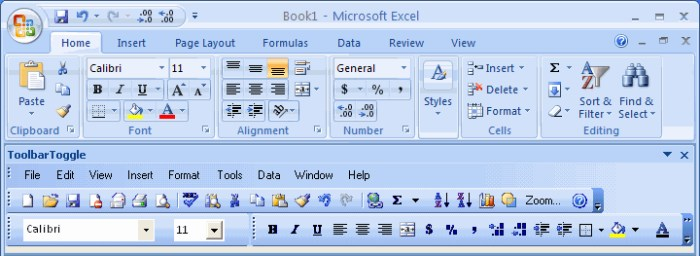
\includegraphics[width=\textwidth]{images/IlComportamentoDegliUtenti-ImplicazioniDellaLeggeDiFitts}
						\caption[Il comportamento degli utenti - Microsoft Office dopo e prima il restyling]{Il comportamento degli utenti - Microsoft Office dopo e prima il restyling}
						\label{fig:ImplicazioniDellaLeggeDiFitts}
					\end{figure}
				
				\paragraph{Complicazioni}
					La legge di Fitts nasce considerando una dimensione, se l'area è uguale (variabile $W$) ma ha forma diversa? Quale pulsante è il migliore? Il pulsante migliore dipende dall'angolo creato dal punto di partenza e la retta. Per cui attenzione!
					
			\subsubsection{Interfacce e Fitts}
				Altri esempi più fini dell'applicazione della legge di Fitts possiamo trovarli già dal primo sistema Macintosh. Il menu è fissato distante, in alto in modo da non avere problemi con l'asse y. Risultato? 5 volte più veloci in media dei menu Windows da qui poi nasceranno le \emph{task bar}. Ancora, lo strumento di \emph{scroll} su Mac ha una barra più lunga e i pulsanti sono vicini al contrario di Windows.
				
					\begin{figure} [h]
						\centering
						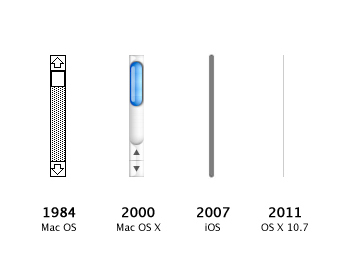
\includegraphics[scale=0.8]{images/IlComportamentoDegliUtenti-InterfacceEFitts}
						\caption[Il comportamento degli utenti - Evoluzione \emph{scrollbar} su Mac]{Il comportamento degli utenti - L'evoluzione della \emph{scrollbar} su Macintosh}
						\label{fig:InterfacceEFitts}
					\end{figure}
				
				\paragraph{Zone magiche}
					Altri suggerimenti che nascono dalla legge di Fitts riguardano i bordi e ancora meglio gli angoli. Essi possono essere utilizzati come pulsanti d'interfaccia super efficaci perché non necessitano del tempo di frenata e l'area dell'obiettivo è molto grande a patto che l'utente non abbia una finestra ridotta sullo schermo. La figura ~\ref{fig:InterfacceEFitts} mostra esplicitamente come il sistema operativo Os X abbia sfruttato queste zone magiche per la \emph{scrollbar}. 
				
				\paragraph{Menu 2.0}
					Anche nei menu possiamo vedere molti usi della legge di Fitts.
					\begin{description}
						\item[Menu a pop-up:] è un'estremizzazione di Fitts, abbiamo i pulsanti vicinissimi al cursore del mouse.
						\item[Menu circolare:] un evoluzione del \emph{menu a pop-up}, può esser completo (\emph{pie menu}) o solo in parte, da usare negli angoli soprattutto (\emph{fan menu}).
					\end{description}
					Tra i \emph{pie menu} e i \emph{menu lineari} non c'è dubbio che sull'usabilità vincono i primi, ma non sottovalutiamo i secondi che  per tanti elementi/comandi se combinati assieme ad altri tipi di menu possono dare risultati efficaci.
					Ricordiamo che i primi software ad implementare i menu 2.0 sono stati i videogame, l'uso del \emph{pie menu} in \emph{Second Life} (figura ~\ref{fig:PieMenu}) lo portò ad un gran successo. In altri l'uso dei \emph{pie menu} permetteva di essere rapidi nel eseguire comandi attraverso movimenti del mouse che aprivano catene di \emph{pie menu}.
				
				\begin{figure}
				\centering
					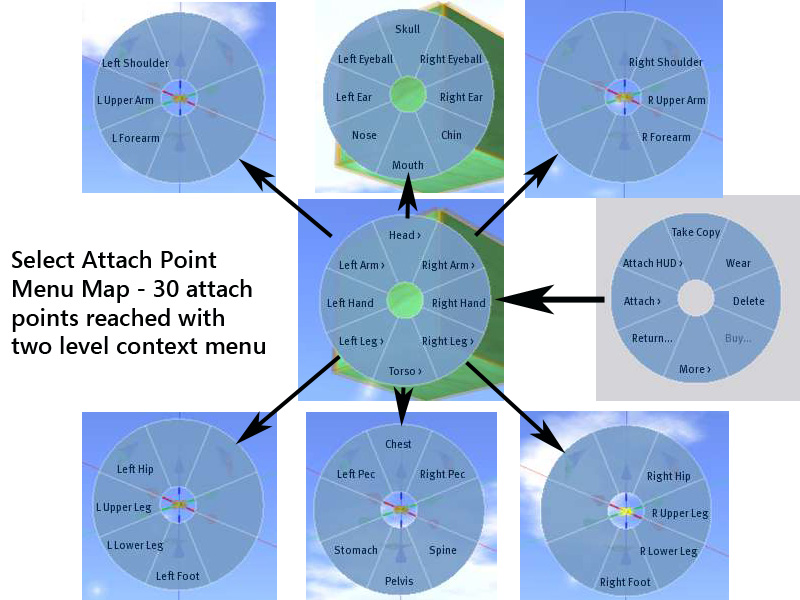
\includegraphics[width=\textwidth]{images/IlComportamentoDegliUtenti-PieMenu}
					\caption{Il comportamento degli utenti - Pie menu su \emph{Second Life}}
					\label{fig:PieMenu}
				\end{figure}